\documentclass{article}
\usepackage[english]{babel}
\usepackage[utf8]{inputenc}
\usepackage{amsmath}
\usepackage{array}
\usepackage{newtxtext}
\usepackage{newtxmath}
\usepackage{color}
\usepackage{textcomp}
\usepackage{listings}
\usepackage{caption}
\usepackage{hyperref}
\usepackage{multicol}
\usepackage{lmodern}
\usepackage{graphicx}
\usepackage{xcolor}
\usepackage{soul}

\usepackage[top=2cm, bottom=2cm, left=2cm, right=2cm]{geometry}

\newcommand{\maintitle}{LINGI2255\\
\vspace{0.5\baselineskip}
Software Development Project\\     % Titre
\vspace{\baselineskip}
{\Large \em Specifications \& Requirements - Team 06}}
\newcommand{\teacher}{Kim \textsc{Mens}} % Professeur
\newcommand{\teachingassistant}{Benoît \textsc{Duhoux}}
\newcommand{\authors}{Youri Mouton, Rémy Voet, Nicola Romano, Sophie Madessis, Samuel Monroe, Antoine Rime, Illias Tchichi} % Auteurs
\newcommand{\HRule}{\rule{\linewidth}{0.5mm}}
\setlength{\parskip}{1ex} % Espace entre les paragraphes

\begin{document}
\newcolumntype{C}{>$c<$}
  % Inspiré de http://en.wikibooks.org/wiki/LaTeX/Title_Creation

\begin{titlepage}

\begin{center}

\begin{minipage}[t]{0.8\textwidth}
  \begin{center}
    
\includegraphics [width=70mm]{logo_ucl.jpg} \\[0.5cm]
  \end{center}
\end{minipage}

\vspace{1cm}

\HRule \\[0.4cm]
{\huge \bfseries \maintitle}\\[0.4cm]
\HRule \\[1.5cm]

\begin{minipage}[t]{0.5\textwidth}
  \begin{center} \large
    \emph{Prof.:} \teacher
  \end{center}
\end{minipage}

\vspace{0.5cm}

\begin{minipage}[t]{0.5\textwidth}
  \begin{center} \large
    \emph{TA:} \teachingassistant
  \end{center}
\end{minipage}

\vspace{0.5cm}

\begin{minipage}[t]{\textwidth}
  \begin{center} \large
    \emph{Auteurs:} \authors
  \end{center}
\end{minipage}

\vfill

{\large 2017-2018}

\end{center}

\end{titlepage}
  \cleardoublepage % Dans le cas du recto verso, ajoute une page blanche si besoin
  \tableofcontents % Table des matières
  \sloppy          % Justification moins stricte : des mots ne dépasseront pas des paragraphes
  \cleardoublepage
  
\section{Module's description}
For the moment the questions are created manually by the professor. To increase the number of questions available for a given skill, we want to give the possibility for a professor to create/solve a large sample of questions based on typical problems.\\
And for the students to efficiently train given skills by exercising on a large set of different problems.\\
It means that first the professor has to create a generic question, for example: $ax^2 + bx + c$ for an equation of the second degree. Then from this generic question we will provide an automatic creation of precise question with  multiple values for a, b and c belonging to natural, integer or rational. We also want to provide some control the domain of the question and answer either integer, rational, complex ...\\

We also need to implement a solver for each type of questions.
The solver should be able to give the students the solution and eventually the resolution step by step of the problem. So that the students knows if he provide the correct answer and can understand his mistake if he has done some. When he is training a given skills.\\

For some problems involving geometrical figures, we would like to implement visualization functionnalities for the student.\\
These functionnalities would take the randomized parameters and display the related figures on the student test.\\
For more advanced shapes or 3D shapes, the visualization functionnalities would provide multiple points of view of these shapes, enabling the best understanding of the shape by the student.\\



%For example let's take the case of the calculation of the perimeter of a circle. Our system will create multiple problems concerning


\section{User stories}

The number before each use story is the value coming from the planning poker session.\\

\begin{enumerate}

    % I want to generate = I want a functionnality to randomly create?
    
    % As a
    % I want to 
    % In order to 
    
    \item 5 :\\ % DONE
    As a teacher\\
    I want to be able to set the domain of a problem\\
    In order to let the question creation functionnalities use this domain for random parameters\\
    
    \item 8 :\\ % DONE
    As a teacher\\
    I want to have, for each assignement topic, a functionnality to create a related problem based on random values\\
    In order to not having to type specific values each time.\\
    
    \item 5 :\\ % DONE
    As a teacher\\
    I want a functionnality to create multiple 2nd degree equations from random values to be solved by students\\
    In order to not having to manually type the parameters\\
    
    \item 3 :\\ % DONE
    As a teacher\\
    I want to be allowed to specify rational, integer or natural answers and parameters for the 2nd degree equations problems\\
    In order to allow the functionnality to use random parameters of different domain types\\
    
    \item 3 :\\
    As a teacher\\ % DONE
    I want a functionnality to create random triangle on which the student will have to compute the perimeter\\
    In order to not having to manually create a triangle for the exercice\\
    
    \item 3 :\\
    As a teacher\\ % NEW user story en lien avec la précédente
    I want to be able to choose how the student should resolve a question, if there are multiple ways to find the answer (e.g. find a triangle's perimeter)\\
    In order to evaluate a specific skill\\
    
    \item 3 :\\
    As a teacher\\ % DONE
    I want a functionnality to create a random triangle on which the student will have to compute the area\\
    In order to not having to manually create a set of triangles\\
    
    \item 2 :\\
    As a teacher\\ % DONE
    I want a functionnality to create a random circle on which the student will have to compute the area\\
    In order to not having to manually create the circles\\
    
    \item 2 :\\
    As a teacher\\ % DONE
    I want a functionnality to create a random quadrilateral/rhombus/square/rectangle/parallelogram/trapezium on which the student will have to compute the perimeter\\
    In order to not having to create them manually\\
    
    \item 2 :\\ % DONE
    As a teacher\\
    I want a functionnality to create a random quadrilateral/rhombus/square/rectangle/parallelogram/trapezium on which the student will have to compute the area\\
    In order to not having to create them manually\\
    
    \item 3 :\\ % DONE
    As a teacher\\
    I want a functionnality to create a random regular polygon (n=5 to 10) on which the student will have to compute the perimeter\\
    In order to not having to create the polygon manually\\
    
    \item 3 :\\ % DONE
    As a teacher\\
    I want a functionnality to create a random regular polygon (n=5 to 10) on which the student will have to compute the area\\
    In order to not having to create the polygon manually\\
    
    \item 2 :\\ % DONE
    As a teacher\\
    I want a functionnality to create a random problem where the student will have to find the length of the side of a triangle (using Pythagoras theorem)\\
    In order to not having to create multiple questions manually \\
    
    \item 5 :\\ % DONE
    As a teacher\\
    I want a functionnality to create a random statistical data on which the student will have to compute characteristic values (one characteristic value for one question)\\
    In order to not having to create them manually\\
    
    \item 2 :\\ % DONE
    As a teacher\\
    I want a functionnality to create a random problem where the student will have to compute the simple interest\\
    In order to not having to manually create that kind of problem\\
         
    \item 3 :\\ % DONE
    As a teacher\\
    I want a functionnality to create a question about compound interest from random values\\
    In order to not having to manually type the parameters of each compound interest problem.\\
    
    \item 13 : \\ % DONE
    As a teacher\\
    I want to have a functionality to select a kind of object (cylinder, cone, prism, pyramid) and create that object from random values to be included in the assignement\\
    In order to not having to specify values for that object, nor including pictures of that object in the test for the student\\

\end{enumerate}

\section{Scenarios}

    \subsection{Assessment for geometry skills}
    
        \begin{enumerate}
        
            \item Professor Layton wants to assess his students about basic geometric 
            skills.
            \item Layton decides to test his students with perimeter and area 
            calculus of triangles (non right-angled).
            \item Layton logs in, reach his class management page and access the 
            assessment creation page.
            \item Layton select the skills for area and perimeter calculus of 
            non right-angled triangles.
            \item Layton creates the assessment.
            \item Questions have been generated with random values ( not leading 
            to extreme shapes of triangle ).
            \item Layton chose to regenerate some of the questions that not 
            fit its tastes.
            \item Layton finalize the test creation, his students can now do it online.
        \end{enumerate}
        
    \subsection{Roots of polynomial assessment}
    
        \begin{enumerate}
            \item Professor Oak decides that the time has come to test his students 
            on determining the roots of a polynomial.
            \item Oak logs in, reach his class management page and access the 
            assessment creation page.
            \item Oak select the said skill in the selection option.
            \item Oak creates the assessment.
            \item Oak is now on the assessment modification page.
            \item Oak chose the type of parameters and answer for the questions 
            related to root calculus.
            \item Oak generate a polynomial and an expected answer with those 
            parameters
            \item Oak validates the test, students can do the assessment online.
        \end{enumerate} 
    \subsection{Assessment for students}
    %TODO 
    %Split the scenario, one for the Assessment and one for training
    
        \begin{enumerate}
        
            \item \hl{Student Sasha has to do the assessment given by teacher Oak.}
            \item \hl{Sasha logs in, reach Assessment section.}
            %\item Sasha chooses a subject that is available.
            \item \hl{Sasha arrives in a Assessment page.}
            \item \hl{Sasha answers at all the exercices given}
            \item \hl{Sasha has finished and leave the assessement.}
            
            % Only for training, show answers after 3 tries
            %\item Sasha see the correction (not resolution) and read feedback
            %\item Sasha can answers again at the exercice and see again the correction.
        
        \end{enumerate}
        
     \subsection{Training for students}
        \begin{enumerate}
            \item \hl{Student Sasha wants to train her skills in a given subject.}
            
            \item \hl{Sasha logs in, reach the training section}
            
            \item \hl{Sasha choose one skills amongst those given by her teacher.}
            
            \item \hl{Sacha arrives in a Training page.}
            
            \item \hl{Sasha try to answer the question, after 3 tries the correction is given.}
            
            \item \hl{Sasha decide she is done training and leave the page.}
        \end{enumerate}
\section{Wireframes}

\subsection{Question Configuration}
The professor can choose subject and assessment type or skills. The right side is the assessment type where he can set the domain radius and parameter.\\
\begin{center}
    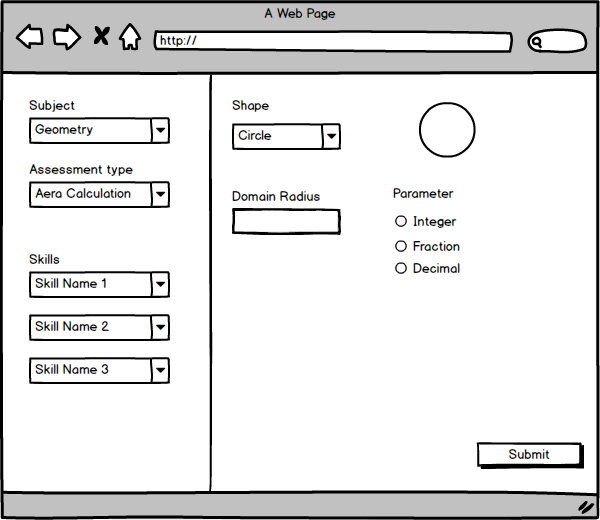
\includegraphics[scale=0.5]{Question_configuration.png}\\
\end{center}
\subsection{Generated Questions Choice}
The professor can choose questions in the list of generated quesions. There is the possibility to generate 5 new question if some are not suitable.\\ 

\begin{center}
    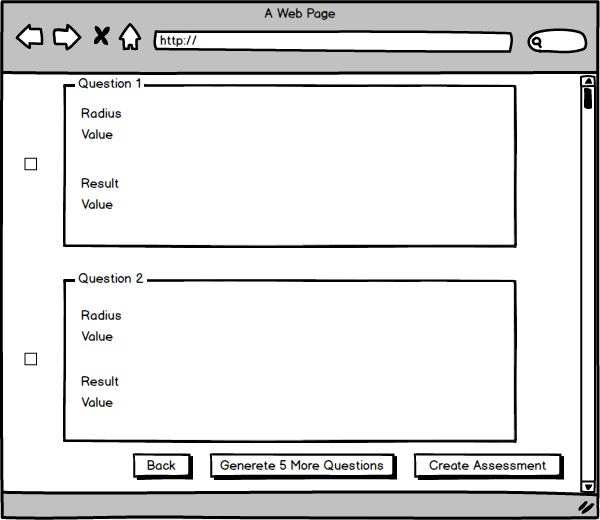
\includegraphics[scale=0.5]{Questions_generated_choice.png}\\
\end{center}
\subsection{Student Answer}
The student has the problem with an illustration and can answer in the input.\\

\begin{center}
    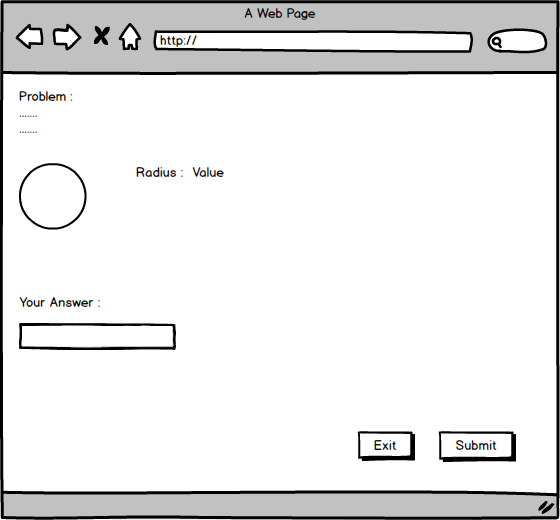
\includegraphics[scale=0.5]{Student_Answer.png}\\
\end{center}
\newpage
\section{Activity diagram}
{\color{red}SPLIT IN TWO PARTS AND FIX SEMANTICS}
Red bubbles in the Activity Diagram highlight the main activities we will be working on.\\
\begin{center}
    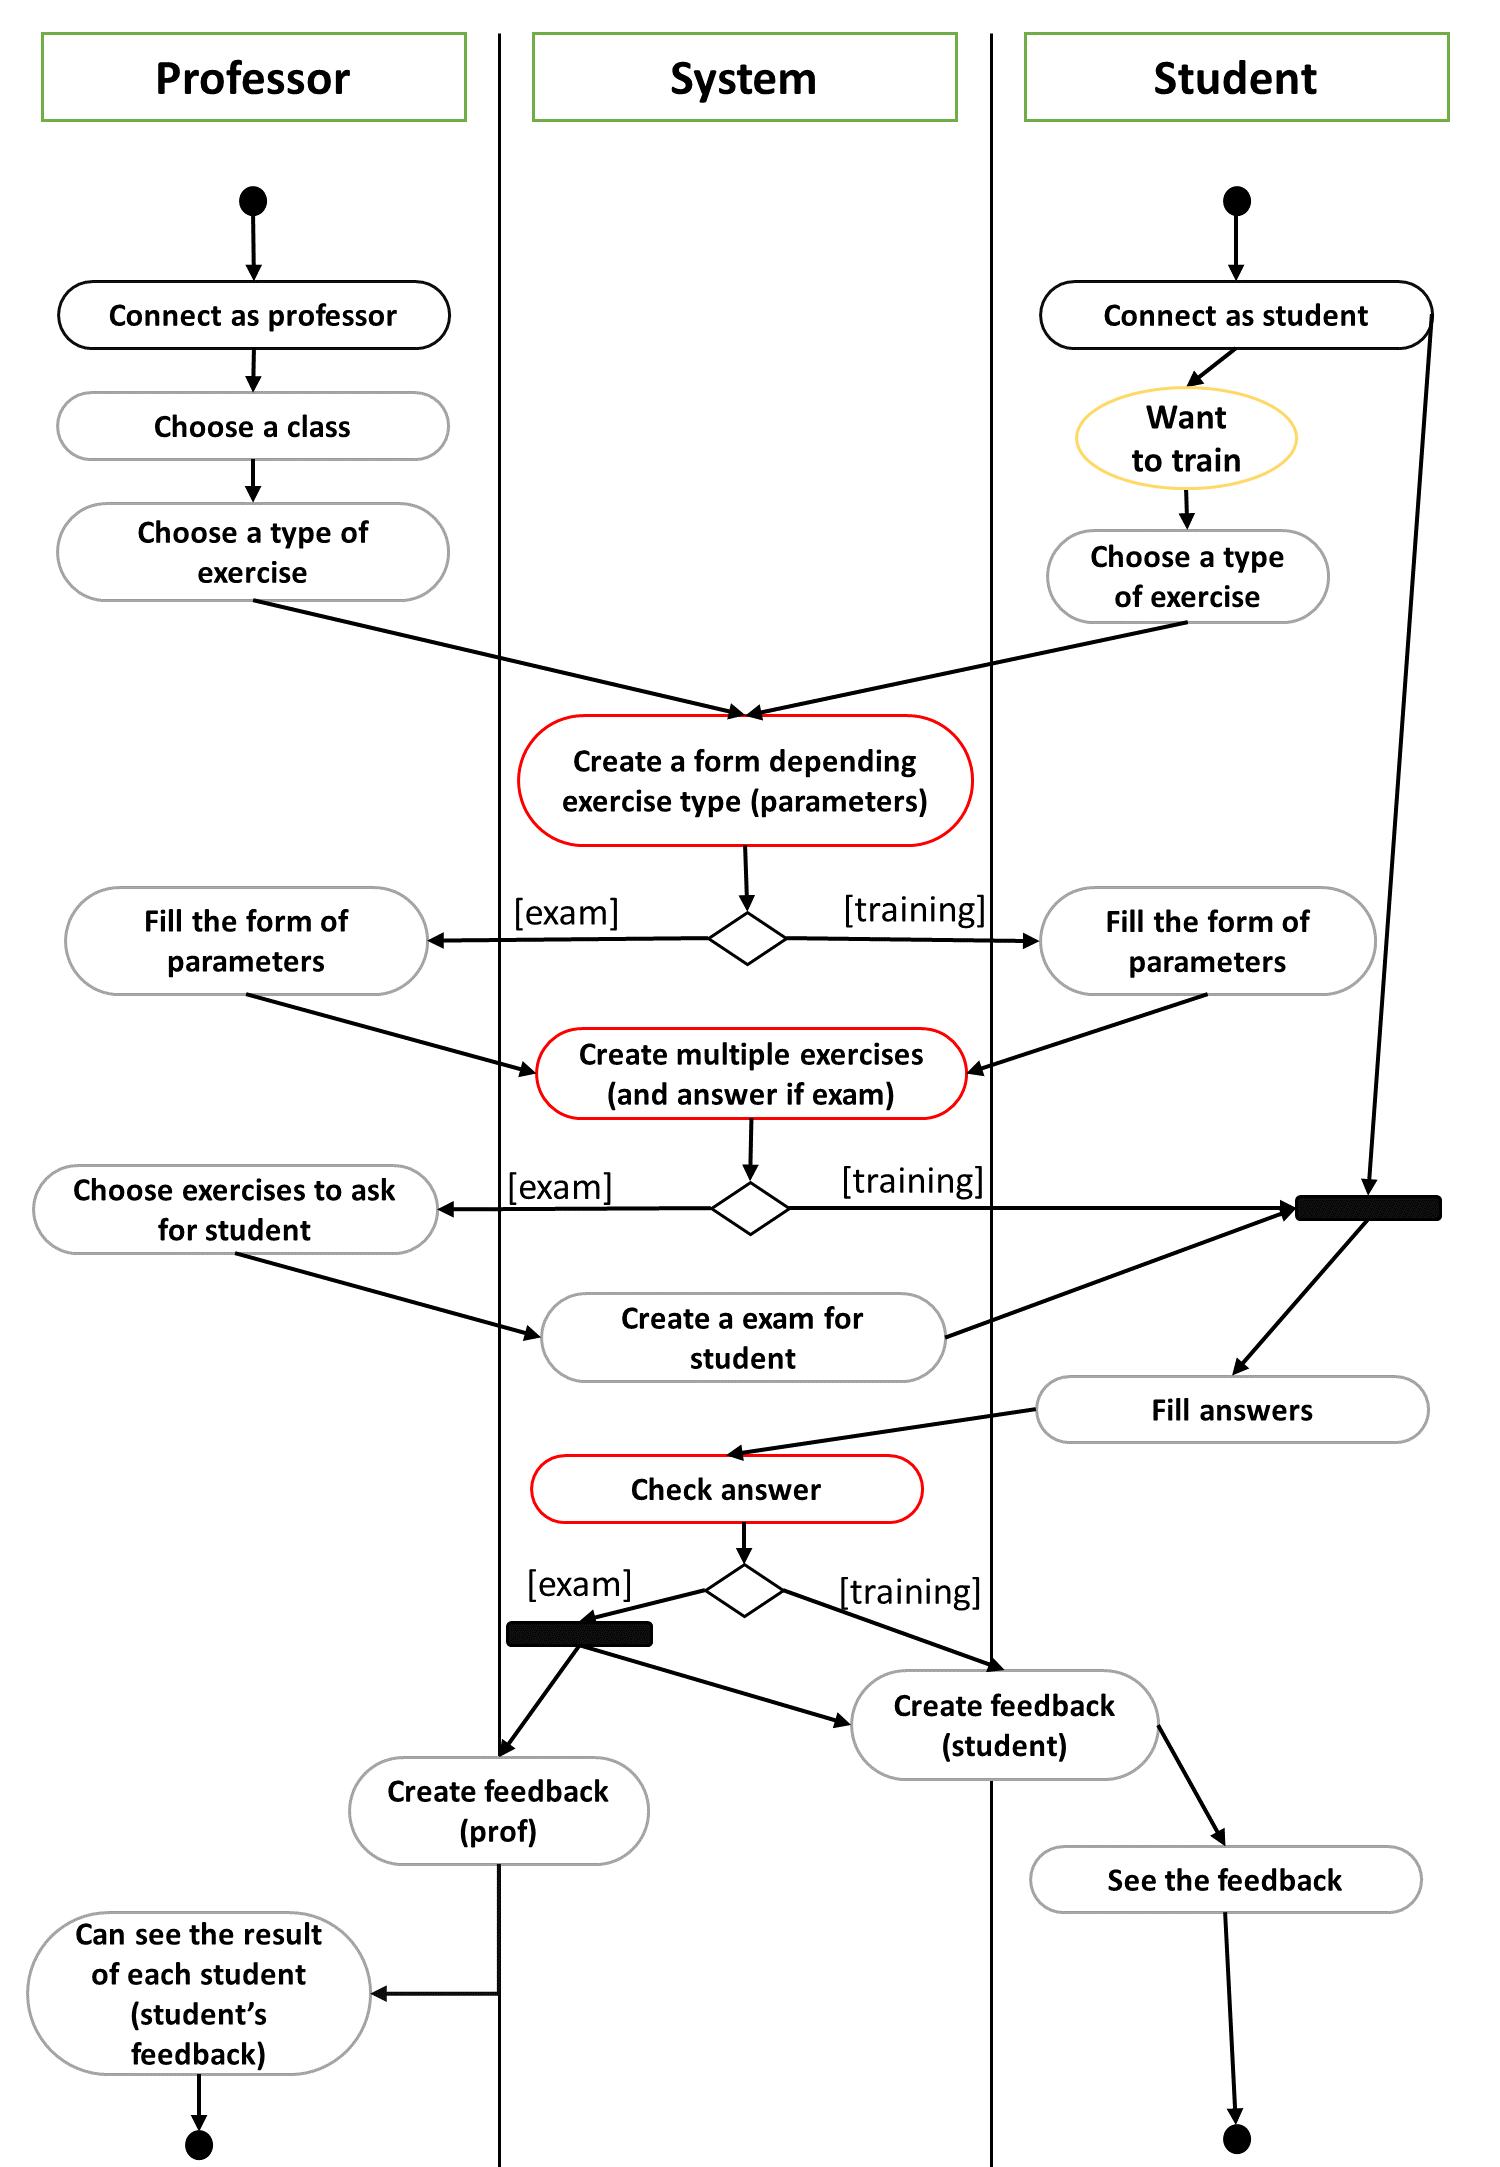
\includegraphics[scale=0.78]{ActivityDiagram.png}
\end{center}
\section{Planning}
\begin{center}
    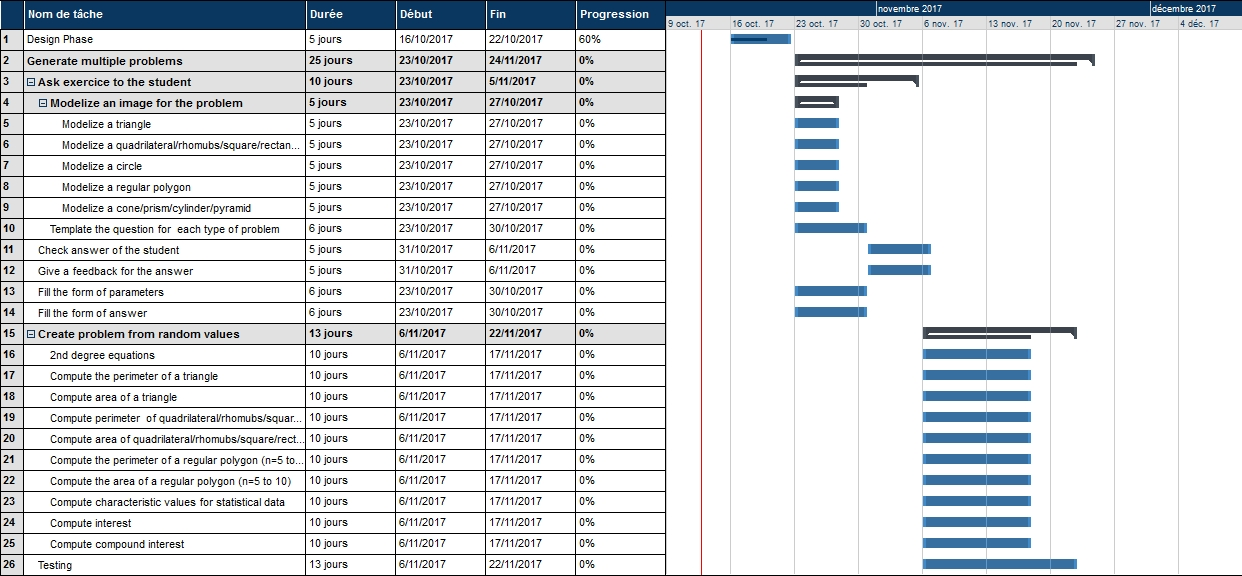
\includegraphics[scale=0.68,angle=90]{multipleproblems.jpg}
\end{center}
\section{Development methodology}
    
    We will be using SCRUM as the Agile methodology.\\
    
    SCRUM suits the best our needs for this project for these reasons : \\
        
        \begin{itemize}
            \item The official planning of the course allows us to organize ourselves 
            in multiple sprints, with personal sub-goals to reach the 
            official deadline.https://www.sharelatex.com/project/59d4d6b5b9df5f5836f753c0
            \item Managing a team of eight people might be really difficult using 
            Waterfall. With SCRUM, everybody is responsible of his own piece of 
            work but also of all the other part of the project.\\
            Nobody's never done with his work and everybody's working towards the 
            same goal, which leads to a stronger "team-spirit".
            \item Frequent stand-up meetings are a good source of motivation, a 
            useful way to keep everybody's knowledge of the project up-to-date.
            \item The team-leader we elected has already responsibilities about
            communications with the clients and team organization, him being the
            SCRUM-Master won't be an overload of work and will perfectly suits the
            whole organization.
            
    \end{itemize}

\section{Organisation and distribution of work in the team}
    
    \begin{itemize}
    
        \item \textbf{Rémy Voet} : Team-Leader, SCRUM Master
        \item \textbf{Sophie Madessis} : Database Engineer
        \item \textbf{Nicola Romano} : Developer, Test Assistant 
        \item \textbf{Youri Mouton} : Lead Developer, Git Master
        \item \textbf{Tristan Moers} : Developer, Team-Leader Assistant
        \item \textbf{Ilias Boutchichi} : Front-End Developer
        \item \textbf{Antoine Rime} : Developer
        \item \textbf{Samuel Monroe} : Behaviour Driven Development, Testing, Front-End Developer
    \end{itemize}
\end{document}https://www.sharelatex.com/project/59d4d6b5b9df5f5836f753c0#section.6